\documentclass[compress,handout,10pt]{beamer}

\newlength{\wideitemsep}
\setlength{\wideitemsep}{\itemsep}
\addtolength{\wideitemsep}{100pt}
\let\olditem\item
\renewcommand{\item}{\setlength{\itemsep}{0.5\baselineskip}\olditem}

\usetheme{berlin}
\usecolortheme{orchid}
\usefonttheme[onlymath]{serif}

\setbeamertemplate{bibliography item}[text]
\usepackage{float}
%\floatstyle{boxed}
\usepackage{colortbl}
\usepackage{mathpazo}
\usepackage{graphicx}
\graphicspath{{./extra/}}
\usepackage{movie15}
\usepackage{bm}
\usepackage{verbatim}
\usepackage{comment}
\usepackage [font=small, labelfont=bf]{caption}
\usepackage{subcaption}
%\captionsetup[subfigure]{labelformat=empty}
\captionsetup[figure]{labelformat=empty}

\newcommand{\mygreen}{\color{green!50!black}}
\newcommand{\myblue}{\color{blue}}
\newcommand{\myred}{\color{red}}
\newcommand{\mycolor}{\color{red}{c}\color{blue}{o}\color{green}{l}\color{orange}{o}\color{cyan}{r}}
\newcommand{\mysize}{\scriptsize{s}\small{i}\normalsize{z}\Large{e}}
\newcommand{\myshape}{\textcircled{s}\textit{h}\texttt{a}\textsf{p}\textsc{e}}

%\xdefinecolor{titlecolor}{rgb}{.855,.647,.125}
%\xdefinecolor{titlecolor}{rgb}{0,0,0}
%\setbeamercolor{frametitle}{fg=titlecolor}
\setbeamerfont{frametitle}{series=\bfseries}
\setbeamercolor{normal text in math text}{parent=math text}

\setbeamertemplate{navigation symbols}{} %gets rid of navigation symbols
\setbeamertemplate{footline}[frame number]
\beamertemplateshadingbackground{blue!5}{yellow!10}

\title{{\LARGE Modeling and Simulating Fan Participation at Large Scale Sporting Events\newline} }

\subtitle{{\large Blue Jays Unlimited} }

\author{ 
%    \vspace{5pt}
    {\bf{Presenters:}}\\ 
Ahmed Aly\\
Steven Su \\
Danni Tang\\ 
    \vspace{5pt}
} 
\institute{JHU AMS 550.400 Fall 2012}
\date{Last Complied on \today} 

\begin{document}

\begin{frame}[plain]
	\titlepage
\end{frame}

\begin{frame}
	\frametitle{Overview}
{\small \tableofcontents}
\end{frame}

\section{Introduction}

\subsection{Background}

\begin{frame}
	\frametitle{The Importance of Cheering in Sports}
		\begin {itemize}
			\item A loud and supportive home crowd is the ultimate home team advantage for sports teams
			\item Home crowd advantage affects the result of the game, shown by past research:
			\begin{itemize}
				\item In US professional sporting leagues, home teams can win approximately 60\% of the time \cite{Jamieson_2010}
				\item In US college athletics, home teams can win approximately 66\% of games played \cite{Snyder_1985}
			\end{itemize}
					\item Home crowd can also improve the ambiance of a sporting event
		\end {itemize}
\end{frame}

\begin{frame}
	\frametitle{What is Cheering?}
		\begin{itemize}
		\item Can show support and enhancing the atmosphere by ``cheering'':
		\begin{itemize}
			\item Chanting the school fight song
			\item Waving a rally towel
			\item Doing the wave
			\item Clapping in general
		\end{itemize}
	\item Cheering is essential at collegiate sporting events; improves experience for both teams and the fans
	\end{itemize}
\end{frame}

\begin{frame}
	\frametitle{The Johns Hopkins Blue Jays}
		\begin{itemize}
			\item The Blue Jays have amassed 47 national championships and 187 conference titles \cite{hopathletic}
			\item The Blue Jays have excelled at many sports including:
			\begin{itemize}
				\item The Men's Lacrosse team has won 44 national championships, most recently in 2007 \cite{hopathletic}
				\item The Men's Swimming team won 32 conference championships, including a streak of 28 consecutive conference championships from 1971-1998 \cite{hopathletic}
				\item The Men's Football and Baseball teams were each conference champions for three consecutive years from 2009-2011 \cite{hopathletic}
		\end{itemize}
	\end{itemize}
\end{frame}

\begin{frame}
	\frametitle{Who are Blue Jays Unlimited?}
		\begin {columns}
			\begin{column}{0.5\textwidth}
				\begin {itemize}
					\item Blue Jays Unlimited (BJU) was established in 1995 \cite{bjuwebsite} by a volunteer group of alumni, friends, and staff
					\item Has more than 3000 active members dedicated to supporting and promoting Johns Hopkins University (JHU) athletics \cite{bjuwebsite}
					\item Official booster club for JHU athletics \cite{bjuwebsite}
				\end {itemize}
			\end {column}
			\begin {column}{0.5\textwidth}
				\begin{figure} [h]
					\begin{center}
						
\includegraphics [width=2in] {BJU.jpg}
						\caption {{\tiny The logo of Blue Jays Unilimited. \textit{Courtesy of: http://www.hopkinssports.com/bluejays-unlimited/}}}
					\end{center}
				\end {figure}
			\end {column}
		\end{columns}
\end{frame}

\begin{frame}
	\frametitle{What Does BJU do for Hopkins?}
	\begin {columns}
		\begin {column} {0.5\textwidth}
		\begin {itemize}
			\item Raised more than \$4 million in funds to improve experience for JHU student athletes and fans alike \cite{bjuwebsite}
			\item Funds provide money for capital projects as well as scholarships and operational endowments \cite{bjuwebsite}
			\item Past projects include renovation of the Newton H.~White Athletic Center and recognition banners for championship teams \cite{bjuwebsite}
		\end {itemize}
	\end {column}
	\begin{column} {0.5\textwidth}
		\begin{figure}
			\begin{center}
				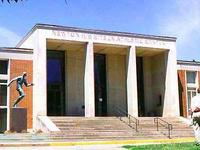
\includegraphics [width=2in] {AthleticCenter.jpg}
				\caption{{\tiny The Newton H.~White Athletic Center after renovations. \textit{Courtesy of: http://events.jhu.edu/WhiteAthleticCenter\#.UHhNK1GRWSo}}}
			\end{center}
		\end {figure}
	\end {column}
\end {columns}
\end {frame}

\begin{frame}
\frametitle{BJU at Sporting Events}
\begin{itemize}
\item BJU is present at nearly all major JHU sporting events
\item Encourage fans to cheer on their Blue Jays to victory in a vociferous and family-friendly manner
\item BJU is interested in maximizing the amount of fan participation in cheering at sporting events to provide the ultimate advantage: a spirited home crowd
\item They believe they can increase fan participation in cheering events by strategically placing student-volunteer ``cheer starters" in the crowd. 
\end{itemize}
\end{frame}

\section{Problem Statement}

\subsection{Official Problem Statement}

\begin{frame}
	\frametitle{Official Problem Statement}
		\begin{itemize}
			\item BJU wants to know if ``cheer starters'' can actually increase cheering and wants a simple model of fan participation in cheering.
		\end{itemize}
\end{frame}

\section {Objectives}

\subsection{Important Details to Consider}

\begin{frame}
	\frametitle {Important Details to Consider}
	\begin {columns}
		\begin {column}{0.5\textwidth}
		\begin{itemize}
			\item Homewood Field's capacity is approximately 8500 spectators \cite{wiki}
			\item Long rectangular section of the bleachers in the lower left is traditionally reserved for Blue Jays' fans and seats approximately 4000 fans
		\end {itemize}
	\end {column}
	\begin {column}{0.5\textwidth}
	\begin {figure}
	\begin{center}
		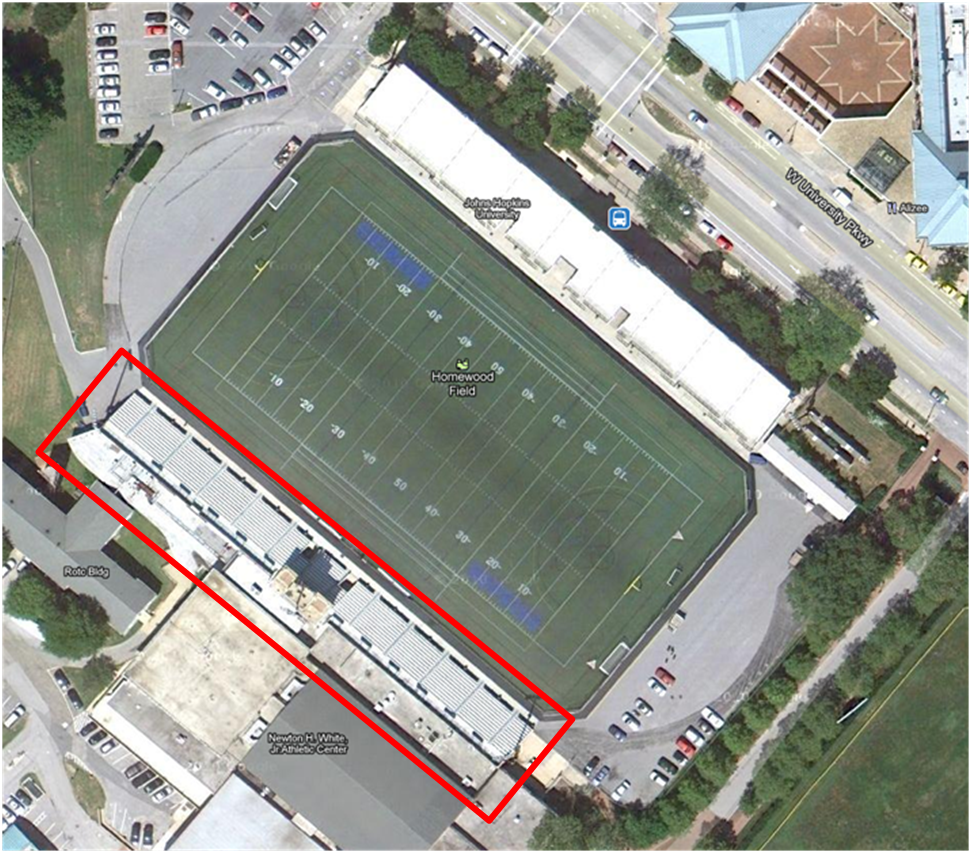
\includegraphics [width=2in] {Bleachers.png}
		\caption {{\tiny A satellite image of Homewood Field. The home team bleachers are highlighted in red. \textit{Courtesy of: www.google.com}}}
		\end{center}
	\end{figure}
\end {column}
\end {columns}
\end{frame}


\begin{frame}
	\frametitle{Important Details to Consider}
	\begin{itemize}
		\item Home bleachers are usually filled to capacity for all major Hopkins sporting events
		\item Because of how fans normally sit, BJU is specifically interested in maximizing cheering in the home team bleachers
	\end{itemize}
\end{frame}

\subsection{Official Objectives}

\begin{frame}
	\frametitle{Objective Statements}
		\begin{itemize}
			\item Provide BJU with a simple model of fan participation in cheering at Homewood Field
			\item Provide simulation results from the model which determine if cheer starters are effective in increasing cheering
			\item If cheer starters are effective, and time permitting, we will provide BJU with details about the quantity and locations at which cheer starters should be placed in order to maximize cheering
		\end{itemize}
\end{frame}

\section{Mathematical Approach and Simulation}
\begin{frame}
\frametitle{Simplifications and Assumptions}
\begin{itemize}
	\item The willingness of a fan in a crowd to cheer depends on:
	\begin{itemize}
	 	\item Number of people cheering around the fan
	 	\item Cheering duration
	 	\item Innate support level
	\end{itemize}
	\item A cheering fan continues cheering until the end of the simulation
	\item The performance of the sports team does NOT influence cheering
	\end{itemize}
\end{frame}

\subsection{Comptutational Simulation}

\begin{frame}
\frametitle{Step 1: Generating Innate Support Level}
\begin{itemize}
\item We generate an arbitrarily sized $n$ x $m$ matrix,
\item  $X$, to represent an $nm$ sized crowd
\item   $X_{ij}$ represents fan $ij$. Each element in $X$ corresponds to fan's innate support level for the team
\item 	Generated by sampling from a normal random distribution with a mean of 10 and a standard deviation of 1 as shown in (\ref{1})
\end{itemize} 
\begin{equation}
X_{ij}\sim Norm(10,1),~\forall~i\in[1,n],~j\in[1,m]
\label{1}
\end{equation}
\end{frame}

\begin{frame}
	\frametitle{Step 1: Generating Innate Support Level}
	\begin{figure}
		\begin{center}
		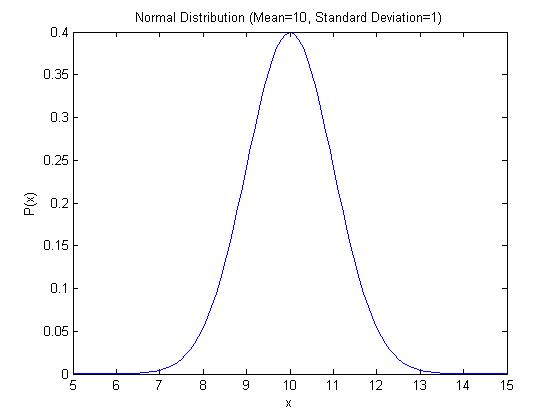
\includegraphics[width=3in] {NormDistribution.jpg}
		\end{center}
		\caption{A Normal Distribution with mean 10 and standard deviation 1}
		\label{fig:normdistribution}
	\end{figure}
\end{frame}

\begin{frame}
\frametitle{Step 2: Determining Which Fans are Initially Cheering}
\begin{itemize}
\item Set an initial threshold, $T_{init}$ to determine which of the fans in the matrix are \textit{initially} cheering
\item A new $n$ x $m$ matrix $X'$ is used to keep track of who is cheering 
\item Elements in $X'$ assigned according to \eqref{2} where 1=cheering and 0=not cheering
\end{itemize}
\begin{equation}
X'_{ij}=1~if~X_{ij}\geq T_{init},~X'_{ij}=0~if~X_{ij}<T_{init}
\label{2}
\end{equation}
\end{frame}


\begin{frame}
\frametitle{Step 3: Including the Influence of Surrounding Fans}
\begin{itemize}
\item $S$ is a $n$ x $m$ matrix stores how many people surrounding a given fan are cheering at a given time
\item Each element in $S$ has corresponding elements with the same row and column indices in both $X$ and $X'$
\item Define a round, $r$, to be the passing of an arbitrary time interval (approximately 3-5 seconds, in this case) 
\end{itemize}
\end{frame}

\begin{frame}
	\frametitle{Step 3: Including the Influence of Surrounding Fans}
		\begin{itemize}
		\item $Y$ is an $n$ x $m$ matrix constructed according to (\ref{3})
		\item Each element in $Y$ represents an individual fan and has corresponding elements in $X$, $X'$, and $S$, with the same row and column indices.	
		\begin{equation}
				Y_{ij}=X_{ij}S_{ij}+r,~\forall~i\in[1,n],~j\in[1,m]
		\label{3}
		\end{equation}
		\item By computing $Y$ as shown in (\ref{3}), the likelihood of a fan starting to cheer increases with the number of surrounding cheering fans and their cheering duration.
		\end {itemize}
\end{frame}	 

\begin{frame}
\frametitle{Step 4: Compare Y to Absolute Threshold and Update Matrices}
\begin{itemize} 
\item Elements in $Y$  are compared to an absolute threshold, $T_{absolute}$ \newline
	\begin{itemize} 
		\item We update $X'$ according to (\ref{4})
		\begin{equation}
			X'_{ij}=1~if~Y_{ij}\geq T_{absolute}
			\label{4}
		\end{equation}
		\item If the individual's score in $Y$ is less than the absolute threshold, corresponding element in $X'$ remains 0  
\end{itemize}
\end{itemize}
\end{frame}

\begin{frame}
\frametitle{Step 5: Repeating Rounds}
To simulate the passing of time:
	\begin {enumerate}
		\item Check to see if any new fans join cheering
		\item Update matrices (i.e.~$X'$ and $Y$)
		\item Repeat steps 2 and 3 for $R$ rounds
	\end {enumerate}
\end{frame}

\section{Results}

\begin{frame}
	\frametitle{Final Parameter Values}
	\begin{itemize}
		\item Rows, $n=20$
		\item Columns, $m=100$
		\item Initial Threshold, $T_{init}=11$
		\item Absolute Threshold, $T_{absolute}=46$
		\item Rounds, $R=10$
		\item Number of Cheer Starters, $CS$ (Variable)
	\end{itemize}
\end{frame}

\begin{frame}
\frametitle{Testing Values for $T_{init}$ and $T_{absolute}$}
\begin{center}
\begin{figure}[h]
\begin{tiny}\begin{tabular}{|l|c|c|c|c|c|c|c|c|c|c|}
\hline
\textbf{Round}&1&2&3&4&5&6&7&8&9&10\\\hline
\textbf{$T_{init}=10$, $T_{abs}=46$}&49.7&74.2&87.15&93.8&97.4&98.85&99.95&99.95&99.95&99.95\\\hline
\textbf{$T_{init}=11$, $T_{abs}=65$}&15.1&15.1&15.15&15.15&15.2&15.35&15.4&15.55&15.65&15.75\\\hline
\textbf{$T_{init}=11$, $T_{abs}=60$}&15.95&16.1&16.15&16.2&16.3&16.4&16.45&16.65&16.75&17.05\\\hline
\textbf{$T_{init}=11$, $T_{abs}=40$}&15.5&21.2&29.15&39.35&52&65.15&76.85&85.5&91.4&95.35\\\hline
\textbf{$T_{init}=11$, $T_{abs}=46$}&15.5&16.65&18.05&20&23.15&27.8&34&42.2&52.2&63.8\\\hline
\end{tabular}
\end{tiny}
\caption{{\tiny Percent of cheering crowd over rounds for some combinations of $T_{init}$ and $T_{absolute}$ values.}}
\end{figure}
\end{center}
\end{frame}

\begin{frame}
	\frametitle{Monte Carlo Simulation}
	\begin{itemize}
		\item For a given $CS$ value, the $CS$ cheer starters were randomly placed in crowd. The crowd simulation was run and the final percentage of cheering fans after 10 rounds was computed as previously described.
		\item For a given $CS$ value this was procedure was repeated for 1000 trials (Monte Carlo Simulation) and the average final percentage of cheering fans after 10 rounds over the 1000 trials was computed. 
		\item Repeated this for $1 \leq CS \leq 50$.
		\item The average final percentage of cheering fans for each $CS$ value was compared to that of when $CS=0$ using a t-test. 
	\end{itemize}
\end{frame}

\begin{frame}
	\frametitle{$CS\geq 39$ Produces Statistically Significant Increase in Cheering}
	\begin{itemize}
		\item When $CS\geq39$, there is a statistically significant $(p<0.05)$ increase in the average final percentage of the crowd who are cheering.
		\item If $CS$ is increased further, the average final percentage of the cheering fans increases, and the p-value decreases.
	\end{itemize}
\end{frame}

\begin{frame}
	\frametitle{Average Final Percentage of Cheering Fans vs Number of Cheer Starters}
	\begin{figure} [h]
		\begin{center}
    			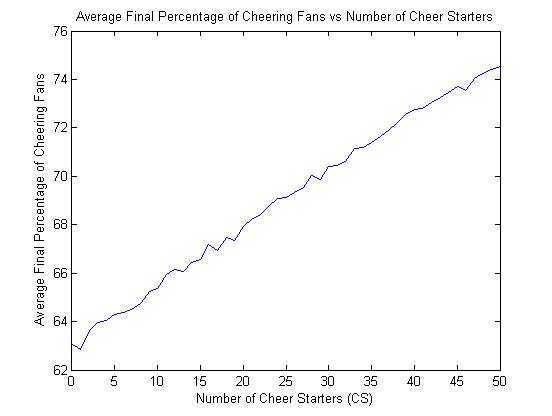
\includegraphics [width=3in] {46(1).jpg}
    			\caption {{\tiny Average final percentage of cheering fans for various $CS$ values.}}
    		\end{center}
    	\end {figure}	
\end{frame}

\begin{frame}
\frametitle{Average Final Percentage of Cheering Fans vs Number of Cheer Starters}
\begin{figure}[h]
\begin{center}
\begin{tiny}\begin{tabular}{|l|c|c|c|c|c|c|}
\hline
\textbf{Number of Cheer Starters}&0&10&20&30&39&50\\\hline
\textbf{Average Final Percentage of Cheering Fans}&63.069&65.346&67.919&70.409&72.533&74.544\\\hline
\textbf{P-value}&0.5&0.34413&0.19637&0.097951&0.047687&0.021585\\\hline
\end{tabular}
\end{tiny}
\caption{{\tiny Average final percentage of cheering fans for various $CS$ values.}}
\end{center}
\end{figure}
\end{frame}

\begin{frame}
	\frametitle{Percent of Cheering Fans Over Time For Various $CS$}
	\begin{figure} [h]
		\begin{center}
    			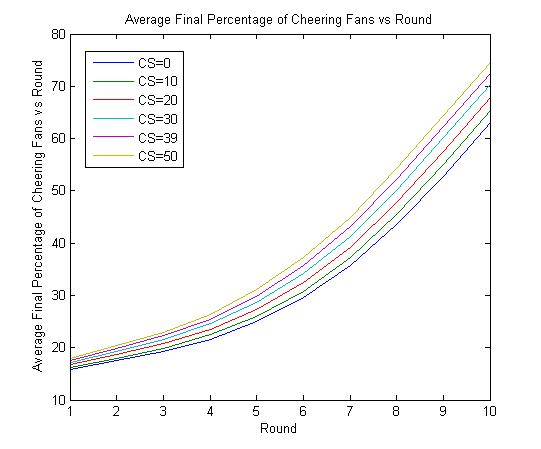
\includegraphics [width=3in] {46(2).jpg}
    			\caption {{\tiny The percentage of cheering fans over time for various $CS$ values.}}
    		\end{center}
    	\end {figure}	
\end{frame}

\begin{frame}
\frametitle{Percentage of Cheering Fans Over Time For Various $CS$}
\begin{figure}
\begin{center}
	\begin{tiny}\begin{tabular}{|l|c|c|c|c|}
\hline
\textbf{Round}&1&3&7&10\\\hline
\textbf{CS=0}&15.875&19.285&35.67&63.069\\\hline
\textbf{CS=10}&16.266&19.936&37.307&65.346\\\hline
\textbf{CS=20}&16.686&20.717&39.246&67.919\\\hline
\textbf{CS=30}&17.13&21.53&41.284&70.409\\\hline
\textbf{CS=39}&17.519&22.261&43.088&72.533\\\hline
\textbf{CS=50}&17.908&23.002&44.936&74.544\\\hline
\end{tabular}
\end{tiny}
\end{center}
\caption{{\tiny The percentage of cheering fans over time for various $CS$ values.}}
\end{figure}
\end{frame}

\begin{frame}
    \frametitle{Visualization of Cheering}
    \begin {columns}
    	\begin{column}{0.5\textwidth}
    		\begin{figure}
    		\begin{center}
    		  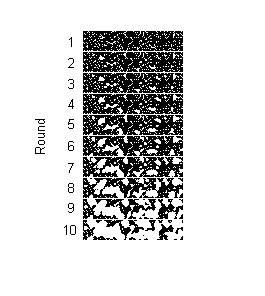
\includegraphics [width=2in] {n=0,46.jpg}
    			\caption {{\tiny Cheering over time when $CS=0$. White indicates cheering.}}
    			\end{center}
    		\end{figure}
    	\end {column}
    	\begin {column}{0.5\textwidth}
    	\begin{figure} [h]
    		\begin{center}
    			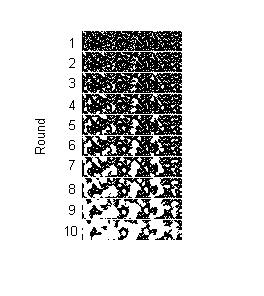
\includegraphics [width=2in] {n=39,46.jpg}
    			\caption {{\tiny Cheering over time when $CS=39$. White indicates cheering.}}
    		\end{center}
    	\end {figure}	
    	\end {column}
    \end{columns}
\end{frame}

\section {Deliverables and Timeline}

\subsection{Deliverables}

\begin{frame}
	\frametitle{Deliverables}
	The model was coded on MATLAB R2009b. All computations were performed on a Intel Core i7 Desktop PC. \newline
	\end{frame}

\begin{frame}
	\frametitle{Checklist of Deliverables}
	From Team to Sponsor:
	\begin {itemize}
	\item MATLAB R2009b and R combination package with test scripts that can be used to reproduce our numerical and simulation test results (In Final Stages)
		\item Technical report and presentations summarizing the work (In Final Stages)
	\item If time permits, a list of patterns of cheer starter setups (i.e.~the number of cheer starters and location of them) that maximize fan cheering (Future Research Recommendations)
	\end{itemize}
\end{frame}

\begin{frame}
	\frametitle{Checklist of Deliverables}
	From Sponsor to Team:
	\begin{itemize}
		\item Timely responses to inquiries (Responses have been timely)
	\end{itemize}
\end{frame}

\subsection{Timeline}

\begin{frame}
	\frametitle{Timeline of Milestones}
	\begin{itemize}
    \item Final Presentation due Nov 28, 2012
    \item Final Report and Deliverables due Dec 20, 2012
	\end{itemize}
\end{frame}

\section{Conclusion}

\subsection{Work Remaining to Be Done}

\begin{frame}
	\frametitle{Remaining Work}
	\begin {itemize}
		\item Finalize Matlab/R combination package
		\item Finish Final Report 
		\end {itemize}
\end{frame}

\subsection{Recommendations for Future Research}

\begin{frame}
	\frametitle {Recommendations for Future Research}
	\begin {itemize}
		\item It would be interesting to see if this model could be applied to other social events (concerts, college lectures, theaters, etc.) where there are large crowds and applause is relevant
		\item Attempt to find patterns in cheer starter placements which maximize cheering
	\end {itemize}
\end{frame}

\subsection{}

\begin {frame} [allowframebreaks]
	\frametitle{References}
	\bibliographystyle{ieeetr}
	%\nocite{*}
	\bibliography{extra/biblioWS}
\end {frame}

\begin{frame}
\frametitle{Acknowledgements}
We would like to thank Professor Nam H.~Lee for his support and academic guidance as well as our classmates for their support.
\end{frame}

\begin{frame}
	\frametitle {Questions?}
	\begin{center}
		Questions?
	\end{center}
\end{frame}

\end{document}
\end{flushleft
